\chapter{統計学}

神の御心を知るには統計学を学ばなければならない(ナイチンゲール)。\\
%{\small この章を学ぶには, 確率の章を既に習得している必要があります。\\}

\section{母集団と標本}

統計学において, 知りたい対象の全ての集合を\underline{母集団}
 (population)\index{ぼしゅうだん@母集団}という。例えば日本の成人男子
の身長がどの程度なのかを知りたいとき, 「日本全国の成人男子全員の身長の集合」
が「母集団」になる。

母集団の中のすべての対象を調べることを「全数調査」という。対象の数が膨大になると, 
全数調査は労力的に大変なので, 母集団から, いくつかの対象(母集団の要素)
を抽出して調べる。このとき母集団から抽出された要素を集めたものを
\underline{標本} \index{ひょうほん@標本}とか\underline{サンプル}(sample)
\index{さんぷる@サンプル}
という。従って, 当然ながら標本(すなわちサンプル)は母集団の部分集合である。
標本を構成する個々の要素(データ)を\underline{標本データ} 
\index{ひょうほんでーた@標本データ}という(言い換えると, 標本は標本データ
の集合である)。このような調査を「標本調査」という。\\

\begin{exmpl}
「日本全国の成人男子全員の身長」を調べるために, 全国から
100人の成人男子を選び出して, 各人の身長を計れば, 100人分の身長のデータ
が得られる。このとき, 100人分のデータをひとまとめにしたものが, 1つの
標本である。1人の身長のデータは「標本」ではなく, 「標本データ」である。
(例おわり)\end{exmpl}
\mv

\begin{q}\label{q:stat_boshudan_def} 母集団とは何か?\end{q}
\mv

\begin{q}\label{q:stat_sample_def} 標本とは何か? 標本と標本データはどう違うか?
\end{q}
\mv

ひとつの標本を構成する標本データの個数を\underline{標本サイズ}とか
\underline{標本の大きさ}とか「サンプルサイズ」という。上の例で言えば, 
100人分の身長のデータから構成される一つの標本について, その
「標本サイズ」は100である。

標本という「集合」がいくつあるか, つまり「標本データのセット」が何セットあるかを
\underline{標本数}とか「サンプル数」という。上の例で言えば, 100人分の身長を計る, 
という操作を, 例えば3回繰り返すと, 100人分の身長のデータが3セット
得られる(つまり300人ぶんの身長のデータが得られる)。この場合, 
標本数やサンプル数は3である(300ではない)。

\begin{freqmiss}{\small\textgt{「標本サイズ」のことを
「標本数」とか「サンプル数」と言ってしまう} ... 間違いです。}\end{freqmiss}

このような間違いをする人や教科書(ウェブ教材等)が多いので大きく
書いておく:

\begin{itembox}{注意!}
標本サイズ(=標本の大きさ=サンプルの大きさ)を
標本数(=サンプル数)と言わないように!
\end{itembox}

用語は正しく使おう。\\


\begin{q}\label{q:stat_size_num_def} 「標本サイズ」と「標本数」はどう違うか?
\end{q}\mv

標本データを母集団の中から\textgt{無作為に抽出する場合}は, 抽出して
みるまではどういう値になるかはわからない。しかし, 母集団の中にたくさん
存在するような値が, 高い確率で標本データに現れるだろう。ということは, 
標本を構成する個々の標本データは, どういう値になるか, 確率的に決まっている。
従って, 標本を構成する個々のデータは1つ1つが「確率変数」と考えることができ, 
それらは同じ確率分布に従っていると考えることができる。その期待値と分散をそれぞれ
\underline{母平均}\index{ぼへいきん@母平均}, 
\underline{母分散}\index{ぼぶんさん@母分散}と呼ぶ。

ただし, これまで学んだ確率変数の例と少し違って, 標本データについて
は, 確率分布がわかっていないことが多い。例えば, サイコロを投げて出る目の値
を実現値とするような確率変数なら, 3が出る確率は1/6である{\small(サイコロが正しく作られていれば)}。
しかし, 日本の成人男子を1人つれてきたらその身長が1.74 mである, という確率は, 
あらかじめわかっているものではない。というか, そもそもそれを知りたいから
調査するのだ。わかっていなければどうするか? 未知数とするのだ。それら
を未知数として数学的な理論を先に構築してしまう。そして, それを逆にたどることによって, 
限られた測定結果から, なるべく正しい, つじつまのあうような結論を導き出すのが統計学である。\\

\begin{q}\label{q:stat_sample_probV} 標本と確率変数はどういう関係にあるか?\end{q}
\vv



\section{標本平均}

\peref{eq:def_expectation0}で定義された期待値は, その確率変数が出してくる, 
最も「平均的な」実現値なので, 期待値のことを\underline{平均}
\index{へいきん@平均}と呼ぶ人もいる。

ところが, 期待値を求めるには, 各実現値の確率が必要であり, それはサイコロの
ような単純な場合を除けば, 現実的には得られないことがほとんどである。
その代替になるのが, 以下に述べる標本平均である。

今, 標本を$\{X_1, X_2, \cdots, X_n\}$とする($X_k$は標本データ, $n$は標本サイズ)。
標本データの総和を標本サイズで割ったもの, すなわち
\begin{eqnarray}
\overline{X}:=\frac{X_1+X_2+\cdots+X_n}{n}\label{eq:arithmean}
\end{eqnarray}
をこの標本の\underline{標本平均}という。これを単に\underline{平均}
と呼ぶ人もいるが, 上述のように, 期待値を平均と呼ぶ人もいるので, 
混同を避けるために, 平均という言葉はできるだけ使わないのが賢明である。

\begin{exmpl}\label{ex:Dice_Sample_mean}
サイコロを8回振って, 出た目が
\begin{eqnarray*}2,\, 3,\, 5,\, 3,\, 6,\, 1,\, 4,\, 5\end{eqnarray*}
だったなら, その標本平均は
\begin{eqnarray*}
\overline{X}=\frac{2+3+5+3+6+1+4+5}{8}=3.625
\end{eqnarray*}
となる。
(例おわり)\end{exmpl}

期待値と標本平均はどのように違うのだろうか? まず, 期待値は, ひとつの定数である。一方, 
標本平均は, それ自体が確率変数である。なぜなら, 個々の標本データが確率変数であるため, 
それを複数個, 足したものも確率変数であり, それを標本サイズ($n$)で割ったものも
確率変数である(一般に, 確率変数どうしの和や定数倍は確率変数だった)。従って, 
標本平均は, 標本をとるたびに微妙に違う値になる。つまり, 標本平均の値は, 標本を
とってみなければわからないのだ。

また, 期待値は, 定数とは言いながら, その値は, 多くの場合は人間にとって永遠に未知である。
しかし標本平均は, 標本が得られれば具体的に一つの値が定まる。\\

ところが, 標本サイズ$n$が十分に大きくなれば, 標本平均と期待値は, 限りなく接近するのだ。
それを確認しよう:

いま, 確率変数$X$が, $x_1,\, x_2,\, \cdots,\, x_N$という, $N$とおりの実現値をとり得るとする。
例えば上のサイコロの例\ref{ex:Dice_Sample_mean}なら$N=6$であり, $x_1=1,\, x_2=2,\, \cdots,\, x_6=6$である。

$n$回の試行\footnote{$n$と$N$を混同しないように!}によって
標本$\{X_1, X_2, \cdots, X_n\}$が得られ, その中で, 値が$x_k$に等しいものが$m_k$
個あったとしよう($k$は1から$N$までの任意の整数である)。それぞれの値をとったデータの数を合計すると, 
標本サイズ, つまり$n$になるので, 
\begin{eqnarray}m_1+m_2+\cdots+m_N=n\end{eqnarray}
である。上のサイコロの例だと, $n$はサイコロを投げた回数, つまり8である。また, 
\begin{eqnarray*}
&&m_1=1,\, m_2=1,\, m_3=2,\\
&&m_4=1,\, m_5=2,\, m_6=1
\end{eqnarray*}
であり, $m_1+m_2+\cdots+m_6=8$である。

また, 全ての標本データの合計は, それぞれの実現値に, その実現値をとった標本データの数をかけたものの和に等しいので, 
\begin{eqnarray}
X_1+X_2+\cdots+X_n=x_1m_1+x_2m_2+\cdots+x_Nm_N\nonumber\\
\label{eq:mean02}
\end{eqnarray}
である。上のサイコロの例だと, この左辺は
\begin{eqnarray*}2+3+5+3+6+1+4+5\end{eqnarray*}
であり, 右辺は
\begin{eqnarray*}1\times1+2\times1+3\times2+4\times1+5\times2+6\times1\end{eqnarray*}
であり, ともに29で一致する。

従って, 式(\ref{eq:arithmean})と式(\ref{eq:mean02})より, 
\begin{eqnarray}
\overline{X} &=& \frac{x_1m_1+x_2m_2+\cdots+x_Nm_N}{n}\\
&=&x_1\frac{m_1}{n}+x_2\frac{m_2}{n}+\cdots+x_N\frac{m_N}{n}\label{eq:largenumber01}
\end{eqnarray}
ここで, $m_k/n$は, $n$が十分に大きければ, 実現値$x_k$が起きる確率$p_k$に等しい(これは確率の定義!)。
従って, 上の式(\ref{eq:largenumber01})は, 
\begin{eqnarray}
\fallingdotseq x_1p_1+x_2p_2+\cdots+x_Np_N
\end{eqnarray}
となり, 右辺は期待値の定義式になる。

このように, 標本サイズ$n$が十分に大きければ, 期待値$E[X]$と標本平均$\overline{X}$はほとんど
一致する。従って, 標本平均で期待値を推定することができる。

とはいえ, 標本サイズ$n$を無限に大きくはできないし, そもそも両者は別の
ものなのだから, 期待値と標本平均はきちんと区別すべきである(統計学がわからないという人は, 
得てしてこういうところが雑である)。

\begin{q}\label{q:stat_expect_average_def} 期待値と標本平均の定義をそれぞれ述べよ。\end{q}
\vv

\section{標準誤差と大数の法則}
さて, 先に述べたように, 標本平均$\overline{X}$は, それ自体がひとつの確率変数
なので, $\overline{X}$にも期待値, 分散, 標準偏差があるはずだ。それらを求めてみよう:

いま, 同じ母集団から, 互いに独立に抽出された$n$個の標本データ
\begin{eqnarray}X_1, X_2, \cdots, X_n\label{eq:sample_data_n}\end{eqnarray}
から構成される標本を考えよう。どのデータも同じ母集団から抽出されるので, \eref{eq:sample_data_n}
を, 互いに同じ期待値$\mu$と同じ分散$\sigma^2$を持つ確率変数とみなす。すなわち, 
\begin{eqnarray}
&&E[X_1]=E[X_2]=\cdots=E[X_n]=\mu\\
&&V[X_1]=V[X_2]=\cdots=V[X_n]=\sigma^2
\end{eqnarray}
である。すると, \eref{eq:arithmean}, \peref{eq:stochX_aX_B}, \peref{eq:expect_Xsum}より, 
\begin{eqnarray}
E[\overline{X}]&&=E\Bigl[\frac{X_1+X_2+\cdots+X_n}{n}\Bigr]\nonumber\\
&&=\frac{E[X_1+X_2+\cdots+X_n]}{n}\nonumber\\
&&=\frac{E[X_1]+E[X_2]+\cdots+E[X_n]}{n}\nonumber\\
&&=\frac{\mu+\mu+\cdots+\mu}{n}=\frac{n\mu}{n}=\mu
\end{eqnarray}
従って, 標本平均の期待値は母平均(期待値)に等しい。

次に, 標本平均の分散を調べてみよう: まず, 標本データは互いに独立なので, \eref{eq:V_X_Y_n}より, 
\begin{eqnarray}
&&V[X_1+X_2+\cdots+X_n]
=V[X_1]+V[X_2]+\cdots+V[X_n]\nonumber\\
&&=\sigma^2+\sigma^2+\cdots+\sigma^2=n\sigma^2
\end{eqnarray}
となる。上式と\eref{eq:variance_trans_ab}より, 
\begin{eqnarray}
V[\overline{X}]&=&V\Bigl[\frac{X_1+X_2+\cdots+X_n}{n}\Bigr]\nonumber\\
                &=&\frac{1}{n^2}V[X_1+X_2+\cdots+X_n]=\frac{1}{n^2}n\sigma^2=\frac{\sigma^2}{n}\nonumber\\\label{eq:var_averageX}
\end{eqnarray}
となる。従って, 標本平均の分散は母集団の分散(母分散)を標本サイズで割ったもの
である。

さて, 「標本平均の標準偏差」つまり$\sigma[\overline{X}]$のこと
を\underline{標準誤差}\index{ひょうじゅんごさ@標準誤差} (standard error)
と呼ぶ(定義)。\textgt{標本データどうしが独立ならば}, 標準誤差は
\eref{eq:var_averageX}の最後の項の平方根をとればいい。
その結果, 
\begin{eqnarray}
\sigma[\overline{X}]=\frac{\sigma}{\sqrt{n}}\label{eq:sigma_averageX}
\end{eqnarray}
となる。$n$が大きくなればなるほど, \eref{eq:sigma_averageX}は0に近づく
のは明らかだろう。
すなわち, \textgt{標本データどうしが独立ならば}, 
標準誤差(標本平均の標準偏差)は母集団の標準偏差の$1/\sqrt{n}$になる, 
という性質があるのだ。

標準誤差は, 標本平均がその期待値からどのくらいばらつくか(誤差の大きさ)
の指標になる。\textgt{標本データどうしが独立ならば}, それは
標本サイズの平方根に反比例するのだ。つまり, 標本平均の誤差を1/10に
しようとすれば, 標本サイズは100倍にしなければならないのだ。

以上をまとめると, 次のような法則になる:
\begin{itembox}{大数の法則}\index{だいすうのほうそく@大数の法則}
\textgt{標本データどうしが独立なら}, 標本平均$\overline{X}$は, 
標本サイズ$n$を増やすほど母平均(つまり期待値$E[X]$)に近づく。
母集団の標準偏差を$\sigma$とすると, このときの標準誤差
(標本平均の標準偏差)は, $\sigma/\sqrt{n}$である。
\end{itembox}

\begin{freqmiss}{\small\textgt{大数の法則を述べるときに, 「標本データどうしが独立なら」
という前提条件を忘れる} ... 世の中の統計学の教科書の中にも, 
この条件を明記しないものが多くありますが, この条件は絶対に必要であり, 
決して忘れてはダメです。}\end{freqmiss}

\section{標本分散と標本標準偏差}

前節で, 母集団の平均(期待値)は, 標本平均によって, ひとつの(十分大きな)標本から
推定できることがわかった。では, 母集団の分散はどのようにして推定できるのだろう? 
分散は\peref{eq:defvar}で定義されるのだが, 実際にこの式に基づいて計算するには, 
各実現値の確率が必要であり, 統計学が必要とされるような多くの場合は, それは
現実的には未知である。現実的に標本から計算可能で, しかも\eref{eq:defvar}のかわりになる
ような量は無いだろうか? それがここで学ぶ「標本分散」である。

標本$\{X_1, X_2, \cdots, X_n\}$について
\begin{eqnarray}
s^2:=\frac{1}{n}\sum^{n}_{k=1}(X_k-\overline{X})^2\label{eq:def_var_samp}
\end{eqnarray}
を\underline{標本分散} \index{ひょうほんぶんさん@標本分散}と呼ぶ(定義)。
その(正の)平方根$s$を標本標準偏差\index{ひょうほんひょうじゅんへんさ@標本標準偏差}
と呼ぶ(定義)\footnote{念のため言っておくが, 標本標準偏差は「標本平均の標準偏差」
とは別物である(言葉は似ているけど)。}。\\

標本分散は, \peref{eq:defvar}で
定義される「分散」と, 言葉は似ているが別物である。ただし, 標本が十分に大きければ, 
標本分散は分散の良い推定値になる(ここでは証明しない)。だからといって
\textgt{分散と標本分散を混同してはいけない}。

厳密に言えば, 全数調査でない限り, 分散の推定値としては, \eref{eq:def_var_samp}
ではなく, 次のような量$u^2$を使うほうが, より適切である:
\begin{eqnarray}
u^2:=\frac{1}{n-1}\sum^{n}_{k=1}(X_k-\overline{X})^2\label{eq:def_var}
\end{eqnarray}
この$u^2$を\underline{不偏分散} \index{ふへんぶんさん@不偏分散}という(定義)。
分母が$n$ではなくて$n-1$になっていることに注意せよ。この正体は, 大学の統計学の
授業で学ぶだろう。

\begin{q}\label{q:stat_exam_var0} ある小学校のクラスの児童の学力を調べるために, 
10点満点の試験をしたところ, 各児童の得点$x$は, 以下のとおりであった:
\begin{eqnarray}
3,\, 4,\, 3,\, 5,\, 6,\, 4,\, 5,\, 6,\, 4,\, 7\label{eq:childrendata}
\end{eqnarray}
電卓を使って, 以下の計算を行え:
\begin{enumerate}
\item 標本平均$\overline{X}$は4.7点であることを示せ。
\item 標本分散$s^2$は1.61点$^2$であることを示せ。
\item 標本標準偏差$s$は1.27点であることを示せ。
\end{enumerate}\end{q}
\mv

パソコンの表計算ソフトを使うと, 上の計算が楽にできる。やってみよう。
まず, 表計算ソフトを立ち上げ, スプレッドシートのA列に, (\ref{eq:childrendata})のデータを
以下のように入れる:\\
\begin{tabular}{|>{\columncolor[gray]{0.8}}c|c|c|c|} \hline
\rowcolor[gray]{0.8} & A & B & C \\ \hline
1  & 3  &         &         \\ \hline
2  & 4  &         &         \\ \hline
3  & 3  &         &         \\ \hline
$\cdots$   & $\cdots$ &         &  \\ \hline
10 & 7  &         &  \\ \hline
11 &    &         &  \\ \hline
12 &    &         &  \\ \hline
\end{tabular}\\
\mv

セルA11に, "=sum(A1:A10)/10"と入力する。これで標本平均が計算され, セルA11にその結果が
表示されるだろう。"sum()"というのは, ある範囲内のセルの値を合計するという, 表計算ソフト
特有の関数である。

次に, 各データ$X_k$について, $(X_k-\overline{X})^2$を計算しよう。まず, セルB1に, 
"=(A1-A\$11)*(A1-A\$11)"と入力する。ここで標本平均が入っているセルA11への参照を固定する
ために, 絶対参照を使っていることに注意しよう。そして, このセルB1をコピーして, セルB2から
セルB10までを選んで「ペースト」する。

このB列を合計して, $n$で割って, $s^2$を得よう。そのために, セルB11に, "=sum(B1:B10)/10"
と入れる。この値の平方根が$s$である。それを求めるために, セルB12に, "=sqrt(B11)"と入れる。

この結果, 以下のような表ができるだろう:\\
\begin{tabular}{|>{\columncolor[gray]{0.8}}c|c|c|c|} \hline
\rowcolor[gray]{0.8} & A & B & C \\ \hline
1  & 3   & 2.89    &         \\ \hline
2  & 4   & 0.49    &         \\ \hline
3  & 3   & 2.89   &         \\ \hline
$\cdots$   & $\cdots$ & $\cdots$  &  \\ \hline
10 & 7   & 5.29    &  \\ \hline
11 & 4.7 & 1.61    &  \\ \hline
12 &     & 1.27    &  \\ \hline
\end{tabular}\\

\begin{q}\label{q:stat_exam_var2} 
\begin{enumerate}
\item 上の操作を行って結果を確認せよ。
\item セルA12に, "=average(A1:A10)"と入れてみよ。その結果を標本平均と比較せよ。
\item セルA13に, "=stdevp(A1:A10)"と入れてみよ。その結果を標本標準偏差と比較せよ。
\end{enumerate}\end{q}
このように, 表計算ソフトには, 標本平均や標本標準偏差を求める関数(機能)が備わっている。
\vv

%\begin{q}\label{q:stat_exam_var3} 
%標本$\{X_1, X_2, \cdots, X_n\}$について
%\begin{eqnarray}
%s^2=\frac{1}{n}\sum^{n}_{k=1}X_k^2-(\overline{X})^2\label{eq:def_var_samp5}
%\end{eqnarray}
%が成り立つことを示せ($\overline{X}$は標本平均)。\end{q}



\section{標準化}

確率変数$X$について, 期待値が$\mu$, 標準偏差が$\sigma$であるとき, 
\begin{eqnarray}
\frac{X-\mu}{\sigma}\label{eq:stat_standardize}
\end{eqnarray}
を求めることを\underline{標準化} \index{ひょうじゅんか@標準化}
(又は正規化\index{せいきか@正規化})と呼ぶ(定義)。

\begin{q}\label{q:stat_standardize0}
標準化された確率変数の期待値は0, 分散は1(だから標準偏差も1)になることを示せ。
\end{q}\mv

標準化は, ある標本データについて, 母集団の分布の中で相対的にどのような
位置にあるかを示すために使われることが多い。$\mu$, $\sigma$
が得られないときは, それぞれ標本平均$\overline{X}$, 
標本標準偏差$s$(もしくは$u$)で代用する。\\

\begin{q}\label{q:stat_standardize2} 現在, 日本で満1才の女児の身長は, 
平均74 cm, 標準偏差2.5 cmであるとする。ある満1才の女児の身長は71 cmであった。この値を標準化せよ。
\end{q}\mv

標準化を, 量の次元という観点で考えてみよう。\pref{sect:stat_EVS_dim}で
見たように, 確率変数と, その期待値と, 標準偏差は, 同じ次元を持つ。
だからこそ, \eref{eq:stat_standardize}の分子にあるような引き算が
可能なのだ。また, \eref{eq:stat_standardize}の分母と分子は同じ
次元を持つ。従って, その比である\eref{eq:stat_standardize}は, 
無次元の量になるのだ。このように, 標準化は, 確率変数を「無次元化」
するという役割も持つ。それによって, 様々な次元を持つ様々な確率変数
どうしを, 「無次元」という次元に統一して, 互いに比較することが
できるのだ。例えば, 「体重」と「身長」は, 全く違う次元の
ものを表している(前者は重さ, 後者は長さ)ので, 比べることはできない。
しかし, それらを標準化してしまえば, 「期待値から標準偏差何個分
離れているか」という統一された見方で, 比較ができるのである。

標準化された確率変数を10倍して50を足したものを
「偏差値」\index{へんさち@偏差値}という(高校時代にお世話になったね!):
\begin{eqnarray}
\text{偏差値}:=50+10\times\frac{X-\mu}{\sigma}
\end{eqnarray}

\begin{q}\label{q:stat_hensachi} 
\begin{enumerate}
\item 問\ref{q:stat_standardize2}の女児の身長の偏差値はいくらか?
\item 君の身長の偏差値を, 同年齢・同性の日本人集団の中で
求めよ。{\small ヒント: 母集団の平均・標準偏差は, 「日本人 身長 平均 標準偏差」
で検索! 身長や年齢について, 自分の数値をレポートに書くことをためらわれる人は, 
架空の数値でも構わない。}
\end{enumerate}
\end{q}
\vv


\section{正規分布}

以下のような確率密度関数で表される確率分布を, 
\underline{正規分布} \index{せいきぶんぷ@正規分布} (normal distribution)とか\underline{ガウス分布}
\index{がうすぶんぷ@ガウス分布} (Gaussian distribution)と呼ぶ:
\begin{eqnarray}
f(x):=\frac{1}{\sqrt{2\pi \sigma^2\,}}\,\exp\Bigl\{-\frac{(x-\mu)^2}{2\sigma^2}\Bigr\}
\label{eq:NormalDist}\end{eqnarray}
$\mu$は確率変数の期待値, $\sigma$は標準偏差である。
この式(\ref{eq:NormalDist})は記憶すること!\footnote{これは複雑な式の
ようだが, よく見てみると, まず, expの中に, \eref{eq:stat_standardize}とよく似た式:
\begin{eqnarray}
\frac{x-\mu}{\sigma}\label{eq:stat_standardize_x}
\end{eqnarray}
が(2乗の形になってはいるが)入っていることに気づく。これは標準化である。(\eref{eq:stat_standardize}
で$X$だったのがここで$x$になったのは, 確率密度関数の変数は確率変数$X$
そのものではなくて, その実現値$x$だからである ... わからない人は確率密度
関数の定義を再確認せよ!)。\pref{sect:func_and_dimless}の\ref{sect:func_and_dimless}節
で述べたように, $\exp$はマクローリン展開されるので, その引数は, 無次元量
でなければならない。\eref{eq:stat_standardize_x}は, その役割を担っている
のである。}

こんな式を暗記する必要は無い, という人もいるが, 
まあそう言わずに暗記せよ。こういう式は, 君のように
頭の柔らかいうちに覚えておくと, あとで良かった, と思う
ものである。

{\small 注: この式の分母の$\sigma^2$を根号の外に出して, 
\begin{eqnarray}
f(x)=\frac{1}{\sqrt{2\pi}\,\sigma}{\,\exp\Bigl\{-\frac{(x-\mu)^2}{2\sigma^2}\Bigr\}}
\end{eqnarray}
と書く教科書もある。もちろんこれは数学的には\eref{eq:NormalDist}と同じである。\\}

期待値が$\mu$, 標準偏差が$\sigma$であるような正規分布のことを, $N(\mu,\sigma^2)$と書き表す。

\eref{eq:NormalDist}のグラフは, $x=\mu$となるときピークを示す($f(x)$が最大となる)。そのピークを
挟んで左右対称な形になる(図\ref{fig:NormalDist})。%←この段落, ヤマサキ追加。ここより後ろの加筆の伏線。2011.0905。
この関数の原型は, \peref{eq:Gauss_func}である。実際, $a=1/(2\sigma^2)$として, 
\eref{eq:Gauss_func}のグラフ(P.\pageref{fig:Gauss_func} 図\ref{fig:Gauss_func})を$x$軸方向に$\mu$だけ平行移動し, 
$y$軸方向に$1/\sqrt{2\pi\sigma^2}$倍したら, \eref{eq:NormalDist}のグラフになる。

\begin{figure}[h]
    \centering
    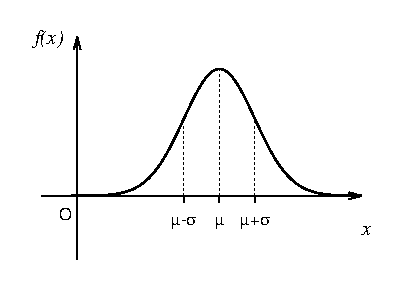
\includegraphics[width=7cm]{normal_dist0.eps}
    \caption{正規分布$N(\mu, \sigma^2)$の確率密度関数。式(\ref{eq:NormalDist})。}\label{fig:NormalDist}
\end{figure}
\mv

\begin{q}\label{q:stat_normal_remember} 正規分布の確率密度関数を表す
式(\ref{eq:NormalDist})を10回書いて, 記憶せよ。
\end{q}\mv

\begin{q}\label{q:stat_normal_remember_integ} 正規分布の確率密度関数, すなわち\eref{eq:NormalDist}
は\eref{eq:probinteq1}を満たすこと, すなわち
\begin{eqnarray}
\int_{-\infty}^{\infty}\frac{1}{\sqrt{2\pi \sigma^2}}\,\exp\Bigl\{-\frac{(x-\mu)^2}{2\sigma^2}\Bigr\}\,dx=1
\label{eq:NormalDist_integ}\end{eqnarray}
が成り立つことを確認しよう。
\begin{enumerate}
\item $t=(x-\mu)/(\sqrt{2}\sigma)$と置いて, 置換積分の公式(\ref{eq:integ_substitute})を使うと, 
\eref{eq:NormalDist_integ}の左辺は次式になることを示せ:
\begin{eqnarray}
\frac{1}{\sqrt{\pi}}\int_{-\infty}^{\infty}e^{-t^2}dt
\label{eq:NormalDist_integ1}\end{eqnarray}
\item ガウス積分の公式(\ref{eq:integ_Gauss_func})を使って, \eref{eq:NormalDist_integ1}は1に等しい
ことを示せ。
\end{enumerate}
\end{q}\mv

\begin{q}\label{q:stat_fig_normal_dist} 以下の正規分布の確率密度関数を, パソコンを使って重ねてグラフに描け。
\begin{edaenumerate}<3>
\item $N(0, 1)$
\item $N(0, 2^2)$
\item $N(1, 1)$
\end {edaenumerate}
\end{q}\vspace{0.3cm}

注意: どのような確率分布でも, 確率密度関数のグラフと$x$軸で囲まれる面積
は必ず1になる。従って, いくつかの正規分布のグラフを重ねて描いたとき, どれかが極端に小さく
なることはありえない。必ず, ピークが下がると横方向に広がる。\\

特に, 期待値が0, 標準偏差が1であるような正規分布, つまり$N(0, 1)$のことを, 
\underline{標準正規分布} (standard normal distribution)と呼ぶ。

\begin{q}\label{q:stat_stdnormal_def} 標準正規分布とは何か?\end{q}
\mv

\begin{q}\label{q:stat_std_normal_dist_f} 標準正規分布$N(0, 1)$
の確率密度関数$f(z)$は, 次式のようになることを示せ:
\begin{eqnarray}
f(z)=\frac{1}{\sqrt{2\pi\,}}\,\exp\Bigl(-\frac{z^2}{2}\Bigr)\label{eq:StdNormalDist}
\end{eqnarray}
注: 普通, 確率密度関数の中の変数は$x$で表すことが多いが, 
標準正規分布に限っては, 変数を$z$で表す慣習である。
\end{q}\vspace{0.3cm}

\begin{figure}[h]
    \centering
    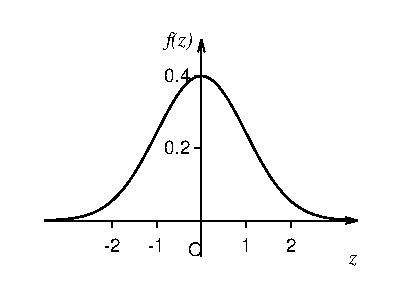
\includegraphics[width=6cm]{normal_dist.eps}
    \caption{標準正規分布$N(0, 1)$の確率密度関数。\eref{eq:StdNormalDist}。}
\end{figure}
\mv

\begin{q}\label{q:stat_std_normal_dist_f_sym} \eref{eq:StdNormalDist}は
偶関数であることを示せ。ヒント: 偶関数の定義に戻って判定する。\end{q}\vspace{0.3cm}

\begin{q}\label{q:stat_normal2std} $N(\mu,\sigma^2)$に従う確率変数$X$を
標準化して得られる確率変数$Z$は, 標準正規分布に従うことを示せ
\footnote{統計学では, なぜか標準正規分布に従うような確率変数を$Z$と書き, 
その実現値を$z$と書く慣習がある。慣習はルールではないので無視
してもいいのだが, 文書を読むときには助けになる。}。\end{q}
\mv

\begin{q}\label{q:stat_int_normal} 標準正規分布に従う確率変数$Z$について, 以下の事実
をパソコンによる数値積分(P.\pageref{sect:suuchisekibun})によって確かめよ。
ヒント:\peref{eq:probdistX1X2}。
\begin{eqnarray}
(1)\,\,\,\, &&P(-1 \leq Z \leq 1)\fallingdotseq 0.683\label{eq:stat_int_normal1}\\
(2)\,\,\,\, &&P(-1.64\leq Z \le 1.64)\fallingdotseq0.90\label{eq:stat_int_normal2}\\
(3)\,\,\,\, &&P(-1.96\leq Z \le 1.96)\fallingdotseq0.95\label{eq:stat_int_normal3}
\end{eqnarray}\end{q}
これらの値は, 後で学ぶ「区間推定」や, いずれ学ぶ「仮説検定」という理論で必要になるので, \textgt{記憶せよ}。

\eref{eq:stat_int_normal1}$\sim$\eref{eq:stat_int_normal3}をグラフ上で表すと, 図\ref{fig:normal_integ}
の上段(塗りつぶした部分)のようになる:
\begin{figure}[h]
    \centering
    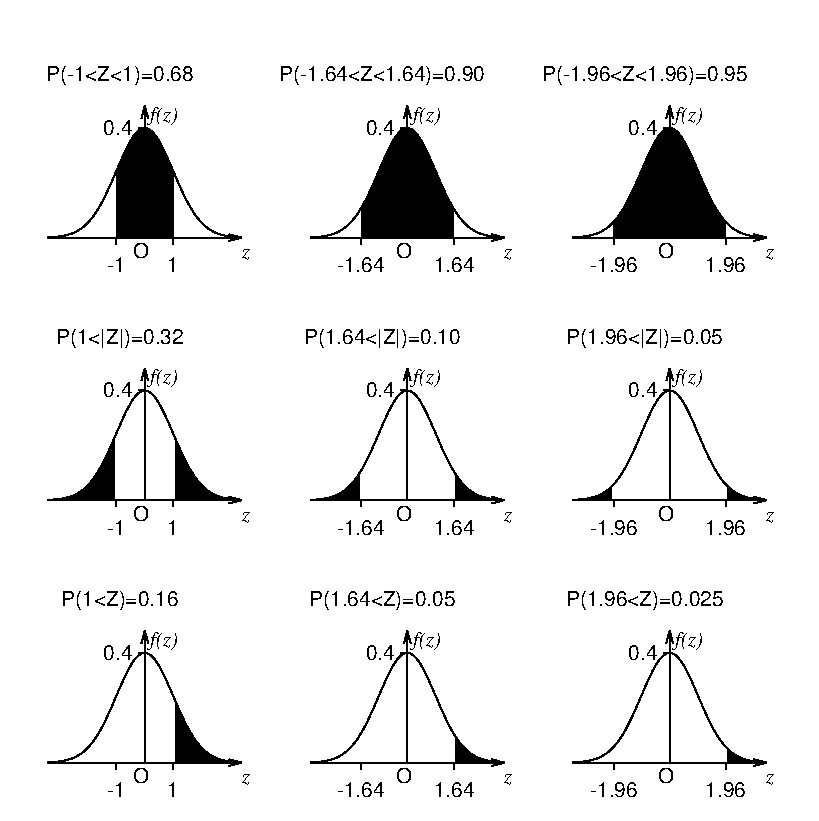
\includegraphics[width=8.5cm]{normal_integ.eps}
    \caption{標準正規分布$N(0, 1)$の確率密度関数と確率の関係。黒く塗りつぶした部分の面積が, 
それぞれのグラフの上部に書かれた確率を表す。}\label{fig:normal_integ}
\end{figure}

図\ref{fig:normal_integ}の中段で塗りつぶされた部分(左右の裾野)
は, 上段で塗りつぶされなかった部分である。それらに対応する確率は, 
1から上段の確率を引いたものになっている。例えば, 中段の左は
$Z$が$-1$以下または$1$以上になる確率(約0.32)を表しているが, それは
1から「$Z$が$-1$以上1以下」になる確率(上段の左; 約0.68)を引いた値に
なっている。

下段で塗りつぶされた部分の面積は, 中段で塗りつぶされた部分の半分である。
各グラフは左右対称(偶関数)だからだ!\\

\begin{q}\label{q:stat_int_normal2} 標準正規分布に従う確率変数$Z$を考える。
図\ref{fig:normal_integ}を用いて, 以下の値を求めよ:
\begin{enumerate}
\item $P(Z \leq 1.64)$
\item $P(Z \leq 1.96)$
\item $P(0\leq Z\leq 1.96)$
%\item $P(2.0< Z)$
\end{enumerate}
\end{q}
\mv

問\ref{q:stat_int_normal}, 問\ref{q:stat_int_normal2}, 図\ref{fig:normal_integ}
は, あくまで, 標準正規分布の話である。正規分布以外の確率分布については, これらの数値は
異なってくる。しかも, 多くの現実的な場合では母集団が従う確率分布がそもそもわからない。
ならばなぜ統計学で正規分布について熱く語るのかというと, 次の「中心極限定理」があるからなのだ。
\vv


\section{中心極限定理}

証明は難しいので省くが\footnote{これを証明するには
今の君の数学力では無理で, フーリエ変換という数学的
技法を駆使して「特性関数」というものを考える必要がある。
それには, 複素数の積分とオイラーの公式が関与している}
, 以下の定理は極めて重要である。

\begin{itembox}{中心極限定理}
母集団がどんな確率分布であっても, 十分に大きな
標本\textgt{の標本平均}は正規分布に従う。
ただし標本データどうしは独立でなければならない。
\end{itembox}
\index{ちゅうしんきょくげんていり@中心極限定理}

\begin{freqmiss}{\small\textgt{上記の中の「の標本平均」という部分を
落として覚えてしまう。} ... 例えば「サイコロを振って出る目の値」
というデータをたくさんとれば, データ自体が正規分布する, 従って, 
連続的な実現値, 例えば2.3とか5.67とかを取りうる, というのですか? 
そんなわけないでしょ。何回振ろうが, サイコロの目は1から6までの
整数値しか取り得ません。}\end{freqmiss}
\mv

\begin{exmpl}\label{ex:cointoss_ntimes_CLT}
コインを1回投げて表の出る回数を$X$とする。$X$は0と1を
実現値とする確率変数で, 期待値$\mu=0.5$, 標準偏差$\sigma=0.5$
である。コインを$n$回投げたときに表が出る割合は, このような確率変数$n$個からなる標本
$\{X_1, X_2, \cdots, X_n\}$
の, 標本平均$\overline{X}$とみなせる。$n$が大きくなれば, $\overline{X}$は
$\mu=0.5$に近づき, その標準偏差は$\sigma/\sqrt{n}=0.5/\sqrt{n}$になる
(大数の法則)。このときの$\overline{X}$の確率分布は, 正規分布$N(0.5, 0.5^2/n)$に近づく。
(例おわり)\end{exmpl}
\mv

大数の法則と中心極限定理は, どちらも標本サイズ$n$が大きくなると
標本平均$\overline{X}$がどうなるかを予測する定理だが, 
大数の法則は, $\overline{X}$が$1/\sqrt{n}$の速さで$E[X]$に
近付くことを主張し, 中心極限定理は, $\overline{X}$の確率分布が
正規分布に近付くことを主張している。両者の違いを区別して記憶せよ。\\

\begin{q}\label{q:stat_CLTdef} 中心極限定理とは何か?\end{q}
\mv

\begin{q}\label{q:stat_CLT_coin10000}
コインを10000回投げて, 表が5100回以上出る確率はどのくらいか?
ヒント: 例\ref{ex:cointoss_ntimes_CLT}で$n=10000$とし, $P(0.51\leq \overline{X})$
を求めればよい。\end{q}
\vv


\section{母平均の区間推定}

統計学を実際の場面で応用する際に, 我々は標本平均$\overline{X}$
によって, 母平均つまり期待値$\mu$を推定しようとする。
そして, 標本サイズ$n$が大きくなるほど, $\overline{X}$は$\mu$に
近づく(大数の法則より)。その「近づく」ということを, より定量的に
表してみよう:

まず, 母集団がどのような確率分布に従うとしても, $\overline{X}$は, 期待値$\mu$, 
標準偏差$\sigma/\sqrt{n}$の正規分布に従う確率変数とみなせる(ここで, 
$\sigma$は母集団の標準偏差)。これは大数の法則と中心極限定理の帰結である。
さて, $\overline{X}$を標準化してできる, 以下のような確率変数$Z$を考える:
\begin{eqnarray}
Z=\frac{\overline{X}-\mu}{\sigma/\sqrt{n}}\label{eq:kukansuitei01}
\end{eqnarray}
問\ref{q:stat_normal2std}より, $Z$は標準正規分布に従う。
従って, \eref{eq:stat_int_normal2}より, 
\begin{eqnarray}
P(-1.64\leq Z\leq 1.64)\fallingdotseq0.90\label{eq:kukansuitei03}
\end{eqnarray}
となる。つまり, 
\begin{eqnarray}
P\Bigl(-1.64\leq\frac{\overline{X}-\mu}{\sigma/\sqrt{n}}\leq1.64\Bigr)\fallingdotseq0.90\label{eq:kukansuitei05}
\end{eqnarray}
となる。\eref{eq:kukansuitei05}の()内の不等式を変形すると, 
\begin{eqnarray}
P\Bigl(\overline{X}-1.64\frac{\sigma}{\sqrt{n}}\leq\mu\leq\overline{X}+1.64\frac{\sigma}{\sqrt{n}}\Bigr)\fallingdotseq0.90\nonumber\\\label{eq:kukansuitei07}
\end{eqnarray}
となる。つまり, 期待値$\mu$は, 90パーセントの確率で, 
\begin{eqnarray}
\overline{X}-1.64\frac{\sigma}{\sqrt{n}}\text{ 以上, かつ }\overline{X}+1.64\frac{\sigma}{\sqrt{n}}\text{ 以下  }\label{eq:stat_shinraikukan90}
\end{eqnarray}
という区間に含まれるだろう, という推定ができるのだ。
このように, 母集団に関する特徴的な値(この場合は母平均$\mu$)を, 「ある確率(この場合は
90パーセント)で, ある区間の中に含まれる」という形で推定することを, 
\underline{区間推定}\index{くかんすいてい@区間推定}という。
その確率(この場合は90パーセント)のことを信頼度\index{しんらいど@信頼度}
と呼び, その区間(この場合は\eref{eq:stat_shinraikukan90})のことを
\underline{信頼区間}\index{しんらいくかん@信頼区間}と呼ぶ。\\

{\small 注: 「$\mu$は90パーセントの確率で, ある区間の中に
含まれる」とは, 具体的にはどういうことだろうか? $\mu$の値が
その区間にふらふらと迷い込んだり出て行ったりするイメージを
持ちやすいが, そうではない。$\mu$の値は, 我々にはわからないが, 
どこかに既に存在して, 静かに座っているのだ。
標本($n$個のデータの集まり)を1つ得れば, \eref{eq:stat_shinraikukan90}
によって「ある区間」が1つ定まる。その区間は, たまたま$\mu$を含む
ようにうまく設定できたかもしれないし, そうでないかもしれない。
そういう「標本を1つとって区間を1つ設定する」という
ことを, 仮想的に何回も(例えば10000回とか)行ったとしたら, その
うち90パーセント(例えば9000回くらい)で, 「設定された区間が$\mu$を含む」
だろう, という意味なのだ。

1つしか標本を得ないのに, たくさんの標本を得るという
状況のことがなぜわかるのだろうか? ポイントは大数の法則である。
標準誤差を標準偏差の$1/\sqrt{n}$で推定できる, 
という定理(\peref{eq:sigma_averageX})
である。その元をたどれば, 独立な確率変数の分散は足し算できるという
定理(\peref{eq:V_X_Y_4})に行き着くのだ。\\}

もっと高い信頼度で推定したい!という場合は, \eref{eq:kukansuitei03}
以降の議論を, 例えば\eref{eq:stat_int_normal3}を使ってやり直せばよい。
すると, 信頼度95パーセントでの信頼区間は
\begin{eqnarray}
\overline{X}-1.96\frac{\sigma}{\sqrt{n}}\text{ 以上, かつ }\overline{X}+1.96\frac{\sigma}{\sqrt{n}}\text{ 以下  }\label{eq:stat_shinraikukan95}
\end{eqnarray}
となり, より広い信頼区間をとらねばならないことがわかる。\\

このように, 母集団の分布が不明でも, 中心極限定理と正規分布
を使えば, 標本平均の「確からしさ」を定量的に検討できるのだ。\\

\begin{q}\label{q:stat_kukansuitei02}
母平均の区間推定において, 同じ信頼度のままで, 信頼区間の大きさを
半分にするためには, 標本サイズを何倍にすればよいか?
\end{q}

この問からわかるように, 一般に, 信頼度を一定にしたままで
信頼区間の大きさを$1/a$倍にしたければ, $a^2$倍の測定回数
をこなさねばならない。例えば, 信頼区間を1/10に縮めたければ, 
測定回数を100倍にしなければいけないのだ!\\

%{\small 注1: 以上の議論は, 標本サイズ$n$が十分に大きいと仮定して中心極限定理を
%使って進めたが, もし母集団が正規分布に従うなら, $n$は大きくなくてもよい。
%というような話が多くの教科書に書いてある。しかし, 現実的には分布の形がわかって
%いるような母集団なんかほとんど無いし, もしあったとしても, そういう対象に
%は統計学なんか使う必要は無い。\\

{\small 注: \eref{eq:stat_shinraikukan90}や\eref{eq:stat_shinraikukan95}を使って
区間推定をする場合, 母集団の標準偏差$\sigma$が必要である。これは, 
普通は未知である(標準偏差が既知であるような母集団なら, 普通, 
期待値だって既知だろう。そこまでわかっていたら統計学なんか使う必要ない)。
その場合, 下の問\ref{q:stat_kukansuitei01}で行うように, $\sigma$は
標本標準偏差$s$や不偏分散の平方根$u$で代用する($s$より$u$を使うほうが正確)。
ただし, その場合, $\overline{X}$は正規分布ではなく, \underline{$t$分布}
\index{tぶんぷ@$t$分布}という確率分布に従うと考える方が, 
より正確な議論になる。実用的には, そちらの方が一般的である。
といっても, 標本サイズが十分に大きければ, 正規分布で考えても
結論はほとんど変わらない。例えば以下の問\ref{q:stat_kukansuitei01}を
$t$分布で考えたとしても, その影響は95パーセント信頼区間の5桁めの
有効数字に現れる程度である。}

\begin{q}\label{q:stat_kukansuitei01}
ある森で, ある種の昆虫(成虫)を, 無作為に400個体採集し, その体長を測ったところ, 
標本平均1.230 cm, 標本標準偏差0.20 cmを得た。この森に棲むこの昆虫(成虫)
の平均的な体長を, 信頼度90パーセントと信頼度95パーセントでそれぞれ区間推定せよ。
ただし, 標本サイズは十分大きいとみなし, 簡単のため, 標準偏差を標本標準偏差で代用せよ。
\end{q}\mv

%\begin{q}\label{q:statistics_English} 以下の言葉を英訳せよ:
%\begin{edaenumerate}<3>
%\item 事象
%\item 背反な
%\item 独立な
%\item 確率
%\item 期待値
%\item 分散
%\item 標準偏差
%\item 確率密度関数
%\item 分布
%\item 母集団
%\item 標本
%\item 正規分布
%\end{edaenumerate}
%\end{q}\mv

\begin{faq}{\small\textgt{いろんな量が正規分布するのはなぜですか?}
... ある量について, 多数の独立な要因が関与し, それらの和や平均としてその量が生じる
としましょう。各要因がどういう確率分布をしても, その和や平均は
中心極限定理によって正規分布します。従って, 多くの要因がからむほど, 
その量は正規分布に従いやすいのです。だからといって, なんでもかんでも
正規分布を仮定してよい, ということではないので, 注意!}\end{faq}

\begin{faq}{\small\textgt{世の中で生きていくためには統計がすごく大事なのに,
高校の授業で扱わないのはヤバいんじゃないですか?!}
... 私もそう思います。}\end{faq}

\vv


\section*{問題の解答}

% 母集団とは何か?
\noindent{\textbf{答}}\ref{q:stat_boshudan_def} 
統計学において, 知りたい対象全体の集合。
\mv

% 標本とは何か?
\noindent{\textbf{答}}\ref{q:stat_sample_def} 
母集団から抽出された要素を集めた集合を標本という。
標本を構成する個々の要素(データ)を標本データという。
\mv

% 「標本の大きさ」と「標本数」はどう違うか?
%2011.07.27 ヤマサキ解答追加。
\noindent{\textbf{答}}\ref{q:stat_size_num_def}
標本という集合を構成する要素(標本データ)の個数を, 
その標本の大きさという。対して, 標本という集合の個数を「標本数」という。
\mv

% 標本と確率変数はどういう関係にあるか?
%2011.07.27 ヤマサキ解答追加。
\noindent{\textbf{答}}\ref{q:stat_sample_probV} 
標本データは確率変数だとみなせる。標本データを集めた集合が標本なので, 標本は確率変数の集合とみなせる。
\mv

% 期待値と標本平均の定義をそれぞれ述べよ。
%2011.0906 ヤマサキ解答追加。
\noindent{\textbf{答}}\ref{q:stat_expect_average_def}
確率変数$X$について, $X$の実現値と, その実現値が発生する確率との積の総和を, $X$の期待値と呼ぶ。

ある標本について, 標本データの総和を標本サイズで割って得られる値を, この標本の標本平均と呼ぶ。
\mv

% ある小学校の6年生児童の学力を調べるために, ...
\noindent{\textbf{答}}\ref{q:stat_exam_var0}  (1) 略。(2) 略。(3) $\sqrt{1.61\cdots}\text{点}\fallingdotseq 1.27$点。
\mv

% パソコンの表計算ソフトを使うと, ...
\noindent{\textbf{答}}\ref{q:stat_exam_var2}  略。
\mv

% 標準化されたデータの期待値は0, 標準偏差は1になることを示せ。
\noindent{\textbf{答}}\ref{q:stat_standardize0} \pref{eq:stochX_aX_B}\eref{eq:stochX_aX_B}
を使って($a=1/\sigma$, $b=\mu/\sigma$とみなして)), 
\begin{eqnarray*}
E\Bigl[\frac{X-\mu}{\sigma}\Bigr]=E\Bigl[\frac{X}{\sigma}-\frac{\mu}{\sigma}\Bigr]
=\frac{E[X]}{\sigma}-\frac{\mu}{\sigma}=\frac{\mu}{\sigma}-\frac{\mu}{\sigma}=0
\end{eqnarray*}
また, \pref{eq:variance_trans_ab}\eref{eq:variance_trans_ab}を使って($a=1/\sigma$, $b=\mu/\sigma$
とみなして),
\begin{eqnarray*}
V\Bigl[\frac{X-\mu}{\sigma}\Bigr]=V\Bigl[\frac{X}{\sigma}-\frac{\mu}{\sigma}\Bigr]
=\frac{V[X]}{\sigma^2}=\frac{\sigma^2}{\sigma^2}=1
\end{eqnarray*}

% 現在, 日本で満1才の女児の身長は, ...
\noindent{\textbf{答}}\ref{q:stat_standardize2}  $(71\text{ cm}-74\text{ cm})/(2.5\text{ cm})=-1.2$
\mv

% 
\noindent{\textbf{答}}\ref{q:stat_hensachi} (1) $50+10\times(-1.2)= 38$。(2) 略。
\mv

% 正規分布の確率密度関数を表す式(\ref{eq:NormalDist})式を10回書いて, 記憶せよ。
%2011.07.27 ヤマサキ, 厳しさの中に優しさとユーモアを追加。
\noindent{\textbf{答}}\ref{q:stat_normal_remember}  がんばれ!
\mv

% 正規分布の確率密度関数, すなわち\eref{eq:NormalDist}は\eref{eq:probinteq1}を満たすこと, 
%2011.07.27 ヤマサキ解答追加。
\noindent{\textbf{答}}\ref{q:stat_normal_remember_integ}
\begin{enumerate}
\item $t=(x- \mu)/(\sqrt2 \sigma)$と置いて, 両辺を$x$で微分すると$dx = \sqrt2 \sigma dt$を得る。また, $t^2=(x- \mu)^2/(2\sigma^2)$。これらを\eref{eq:NormalDist_integ}の左辺に代入すると与式\footnote{ここで, $x \rightarrow \infty$で$t \rightarrow \infty$, $x \rightarrow -\infty$で$t \rightarrow -\infty$なので, 積分区間は変わらない。}を得る。
\item ガウス積分の公式から, 
\begin{eqnarray*}
\frac{1}{\sqrt{\pi}} \int_{-\infty}^{\infty}e^{-t^2}dt
= \frac{1}{\sqrt{\pi}}\,\sqrt{\pi} = 1
\end{eqnarray*}
\end{enumerate}
\mv


% 正規分布の確率密度関数のグラフ
\noindent{\textbf{答}}\ref{q:stat_fig_normal_dist}  図\ref{fig:normal_dist3}。
\begin{figure}[h]
    \centering
    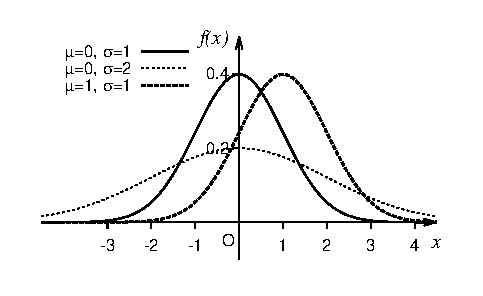
\includegraphics[width=7cm]{normal_dist3.eps}
    \caption{正規分布の確率密度関数\label{fig:normal_dist3}}
\end{figure}
\mv

% 標準正規分布とは何か?
\noindent{\textbf{答}}\ref{q:stat_stdnormal_def} 期待値が0, 
標準偏差が1であるような正規分布, つまり$N(0, 1)$のこと。
\mv

\noindent{\textbf{答}}\ref{q:stat_std_normal_dist_f}
\eref{eq:NormalDist}において, $\mu=0$, $\sigma=1$とすれば与式を得る
(注に従って, $x$は$z$と書き換えればよい)。\\

\noindent{\textbf{答}}\ref{q:stat_std_normal_dist_f_sym} 略。これが
わからない人は, 基礎ができていないので, 勉強法を考えなおすべきである。\\

% $N(\mu,\sigma^2)$に従う確率変数$X$を標準化して得られる確率変数$Z$は, 
\noindent{\textbf{答}}\ref{q:stat_normal2std} $X$を標準化すると, 
\begin{eqnarray}
Z=\frac{X-\mu}{\sigma}\label{q:stat_normal2std_ans0}
\end{eqnarray}
となる。確率密度関数の定義より, 
\begin{eqnarray}
P(x< X\leq x+dx)=\frac{1}{\sqrt{2\pi \sigma^2}}\,\exp\Bigl\{-\frac{(x-\mu)^2}{2\sigma^2}\Bigr\}dx\nonumber\\\label{q:stat_normal2std_ans3}
\end{eqnarray}
である。一方, $X=x$のとき$Z=z$とし, $X=x+dx$のとき$Z=z+dz$とすると, \eref{q:stat_normal2std_ans0}より, 
\begin{eqnarray}
&&z=\frac{x-\mu}{\sigma}\label{q:stat_normal2std_ans35}\\
&&z+dz=\frac{x+dx-\mu}{\sigma}=\frac{x-\mu}{\sigma}+\frac{dx}{\sigma}=z+\frac{dx}{\sigma}\nonumber
\end{eqnarray}
である。従って, 
\begin{eqnarray}
dz=dx/\sigma\label{q:stat_normal2std_ans4}
\end{eqnarray}
である。さて, $x\leq X<x+dx$という事象は$z\leq Z<z+dz$
という事象と同じだから, 
\begin{eqnarray}
P(x\leq X< x+dx)=P(z\leq Z<z+dz)\nonumber\\\label{q:stat_normal2std_ans6}
\end{eqnarray}
となる。\eref{q:stat_normal2std_ans3}, \eref{q:stat_normal2std_ans6}, \eref{q:stat_normal2std_ans35}より, 
\begin{eqnarray}
P(z\leq &&Z< z+dz)=\frac{1}{\sqrt{2\pi \sigma^2}}\,\exp\Bigl\{-\frac{(x-\mu)^2}{2\sigma^2}\Bigr\}dx\nonumber\\
&&=\frac{1}{\sqrt{2\pi \sigma^2}}\,\exp\Bigl(-\frac{z^2}{2}\Bigr)dx
\end{eqnarray}
となる。この右辺の$dx$を\eref{q:stat_normal2std_ans4}によって$\sigma dz$に置き換えると, 
\begin{eqnarray}
P(z\leq &&Z< z+dz)=\frac{1}{\sqrt{2\pi \sigma^2}}\,\exp\Bigl(-\frac{z^2}{2}\Bigr)\sigma dz\nonumber\\
&&=\frac{1}{\sqrt{2\pi}}\,\exp\Bigl(-\frac{z^2}{2}\Bigr) dz
\end{eqnarray}
となる。この右辺の$dz$の係数は, $N(0, 1)$の確率密度関数である。従って$Z$は$N(0, 1)$に従う。\qed
\mv

% 標準正規分布に従う確率変数$x$について, 以下の事実をパソコンによる数値積分によって確かめよ。
%\noindent{\textbf{答}}\ref{q:stat_int_normal} 略。\mv

\noindent{\textbf{答}}\ref{q:stat_int_normal2}  
\begin{enumerate}
\item $P(Z \leq 1.64)$は, 図\ref{fig:normal_integ}の下段中央の
図の白抜きの部分に相当する。塗りつぶされた面積が0.05なのだから, $1-0.05=0.95$。
\item $P(Z \leq 1.96)$は, 図\ref{fig:normal_integ}の下段右の
図の白抜きの部分に相当する。塗りつぶされた面積が0.025なのだから, $1-0.025=0.975$。
\item 図\ref{fig:normal_integ}の下段右の, 右半分を考える。左右対称だから, 
右半分の面積は0.5。そこから塗りつぶされた面積0.025を引いて, $0.5-0.025=0.475$。
あるいは, 図\ref{fig:normal_integ}の中段右の白抜きの面積($1-0.05=0.95$)の半分で0.475
としてもよい。
\end{enumerate}

% 中心極限定理とは何か?
%\noindent{\textbf{答}}\ref{q:stat_CLTdef} 略。\mv

% コインを10000回投げて...
\noindent{\textbf{答}}\ref{q:stat_CLT_coin10000}  表が出る比率$\overline{X}$は, 
今の場合, $5100/10000=0.51$である。中心極限定理により, 
$\overline{X}$は, 近似的には, 平均0.5, 標準偏差$0.5/\sqrt{10000}=0.005$
の正規分布に従うと考えられる。$\overline{X}=0.51$を標準化すると, 
\begin{eqnarray*}Z=\frac{0.51-0.5}{0.005}=2.0\end{eqnarray*}
となる。従って$P(2.0\leq Z)$を求めればよい($Z$は標準正規分布に従う)。
問\ref{q:stat_int_normal}を参考にして数値積分で求めると(あるいは, ネットなどで「正規分布表」を探して参照してもよい), 
$P(2.0\leq Z)\fallingdotseq 0.02??$。従って, 求める確率は約0.02??。(?は伏せ字。自力で導き出せ)
%0.0228
\mv

% 平均値の区間推定において, 同じ信頼度のままで, 信頼区間の大きさを
\noindent{\textbf{答}}\ref{q:stat_kukansuitei02} 標本サイズを$n$とすると, 
信頼区間の大きさは$1/\sqrt{n}$に比例する(\eref{eq:stat_shinraikukan90}や
\eref{eq:stat_shinraikukan95}でわかるように)。従って, 信頼区間の大きさを
1/2倍にするには, $1/\sqrt{n}$を1/2倍にしなければならない。すなわち, 
$\sqrt{n}$を2倍に, すなわち$n$を4倍にしなければならない。
\mv

%ある森で, ある種の昆虫(成虫)を, 400個体採集し, その体長を測ったところ, 
\noindent{\textbf{答}}\ref{q:stat_kukansuitei01}
標本平均$\overline{X}=1.230$~cm, 標準偏差$\sigma\fallingdotseq 0.2$~cm, 
標本サイズ$n=400$匹とする。これらを\eref{eq:stat_shinraikukan90}, 
\eref{eq:stat_shinraikukan95}に代入すればよい。$\sigma/\sqrt{n}=0.2$~cm$/\sqrt{400}=0.01$~cm
であることから, $1.64\sigma/\sqrt{n}=0.0164$~cm, $1.96\sigma/\sqrt{n}=0.0196$~cm。
従って, 母集団の平均$\mu$は, \\
信頼度90パーセントでは, $1.214\text{~cm}$以上かつ, $1.246\text{~cm}$以下\\
信頼度95パーセントでは, $1.210\text{~cm}$以上かつ, $1.250\text{~cm}$以下\\
と区間推定される(ここで, 測定値の有効数字が4桁なので, 信頼区間の上下限の値は5桁目を四捨五入した)。

\begin{freqmiss}{\small\textgt{↑この問題の回答で単位を付け忘れて, $1.214$以上, かつ$1.246$以下, のように書いてしまう。}}\end{freqmiss}

\begin{faq}{\small\textgt{できない問題に限って「略」が多くて困ります}
... 「略」は十分な誘導やヒントが既に与えられている問題です。なので, 自分の頭で
考えて, それを客観的・論理的に表現して下さい。大学の勉強は, 正解を与えられて
そのとおりにやるものではありません。多少表現が違っても, 本質的に正しければ
良いのです。わからなければ, 個別に質問に来てください。「質問する勇気」を養うことも
「略」の狙いです。}\end{faq}
